\documentclass[class=report, float=false, crop=false]{standalone}
%  \usepackage[subpreambles=true]{standalone}

\usepackage{pgf, tikz}
\usetikzlibrary{shapes.misc}
\usetikzlibrary{decorations.pathreplacing}

\tikzset{cross/.style={cross out, draw=black, minimum size=2*(#1-\pgflinewidth), inner sep=0pt, outer sep=0pt},
%default radius will be 1pt. 
cross/.default={0.25pt},
    point/.style={
    thick,
    draw=black,
    cross out,
    inner sep=0pt,
    minimum width=4pt,
    minimum height=4pt,
    },
}

\graphicspath{{figures/figs/}}

% \begin{cbunit}

\begin{document}

\chapter{Results and discussion}
\label{chap:results}

\section{Preliminary results}

Preliminary simulations were performed with only 64 particles, first to ensure that our models and methods were effective and gave realistic results, then to determine what phenomena were different with ellipsoids than with spheres. Simulations performed with this few particles have the advantage to quickly give results to analyse, however finite-size effects are not negligible and can affect the jamming transition (see part \ref{finite-size_effects}).

\subsection{Rheological transition}
\label{preliminary_rheological_transition}

\begin{figure}[h!]
\centering
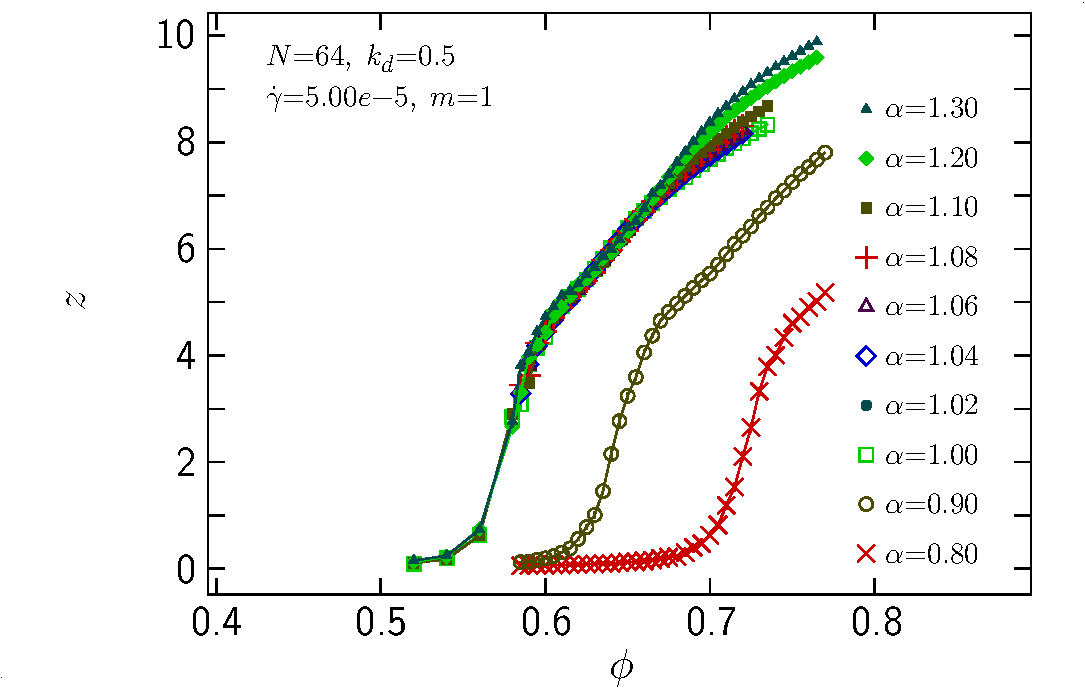
\includegraphics[width=0.6\textwidth]{figures/figs/z_phi_0064_KDk500_Ml100_GDg500}
\caption{Average contact number per particle as a function of the packing fraction for aspect ratios $0.8\le\alpha\le1.3$. $N=64,~ k_d=0.5,~ \dot{\gamma}=5e-5,~ m=1$.}
\label{z_phi_0064_KDk500_Ml100_GDg500}
\end{figure}

\begin{figure}[h!]
\centering
    \begin{subfigure}[t]{0.32\textwidth}
        \centering
        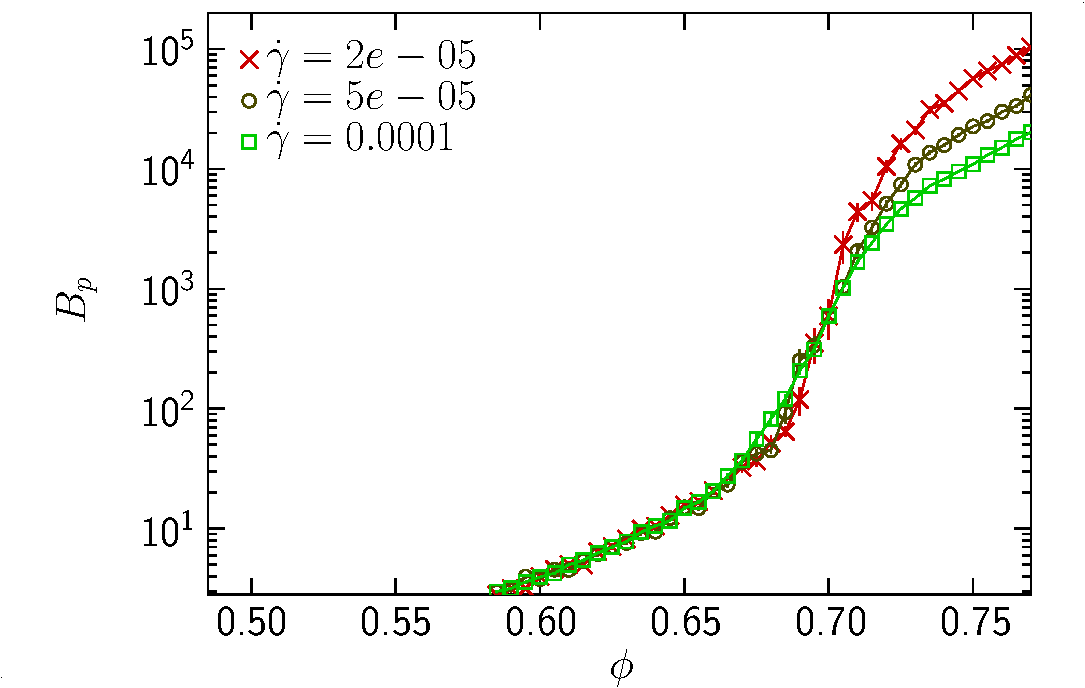
\includegraphics[width=\textwidth]{figures/figs/bp_0064_KDk500_Ml100_EL080}
        \caption{$\alpha=0.8$, $\phi_C\sim0.72$}
        \label{bp_0064_KDk500_Ml100_EL080}
    \end{subfigure}
    \hfill
    \begin{subfigure}[t]{0.32\textwidth}
        \centering
        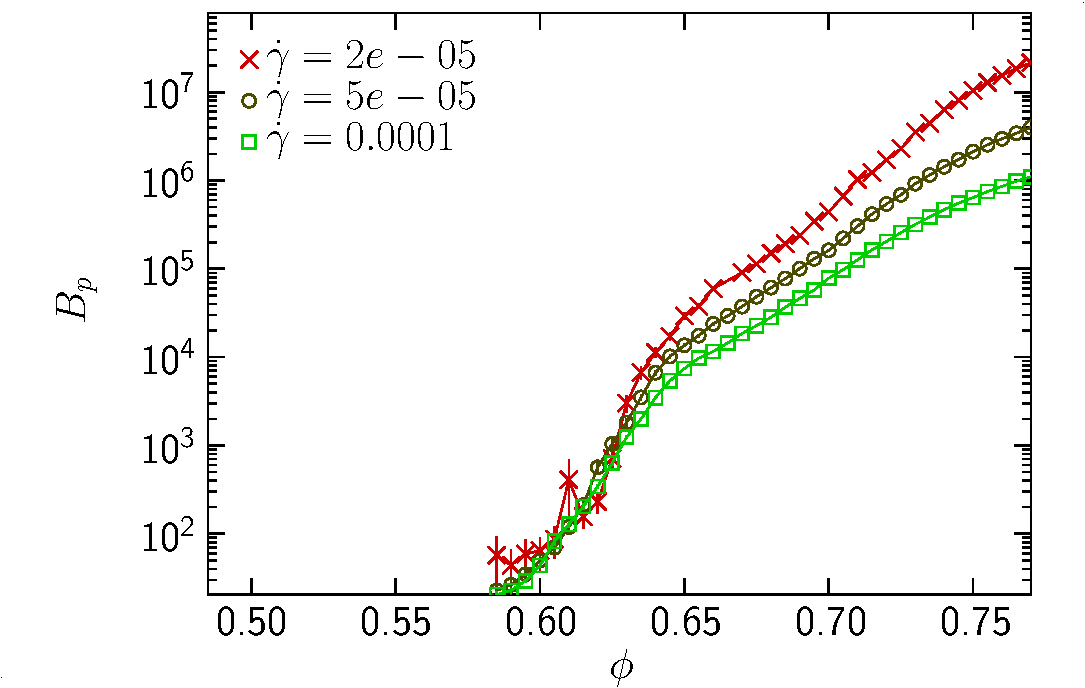
\includegraphics[width=\textwidth]{figures/figs/bp_0064_KDk500_Ml100_EL090}
        \caption{$\alpha=0.9$, $\phi_C\sim0.63$}
        \label{bp_0064_KDk500_Ml100_EL090}
    \end{subfigure}
    \hfill
    \begin{subfigure}[t]{0.32\textwidth}
        \centering
        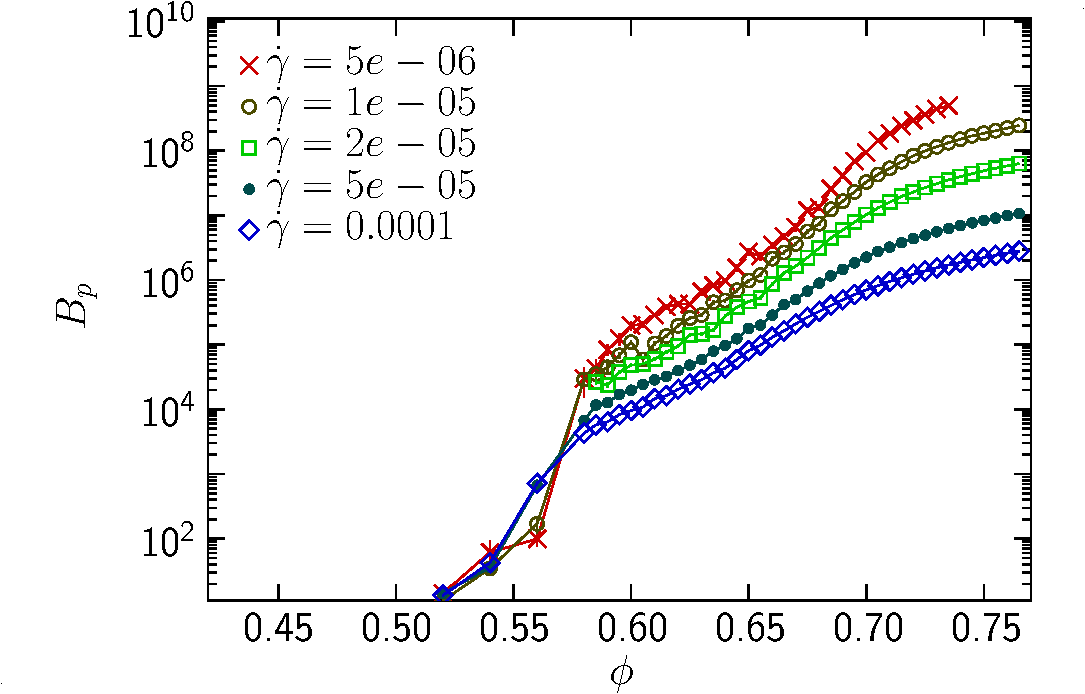
\includegraphics[width=\textwidth]{figures/figs/bp_0064_KDk500_Ml100_EL130}
        \caption{$\alpha=1.3$, $\phi_C\sim0.57$}
        \label{bp_0064_KDk500_Ml100_EL130}
    \end{subfigure}
    
    \vspace{0pt}
    \begin{subfigure}[t]{0.32\textwidth}
        \centering
        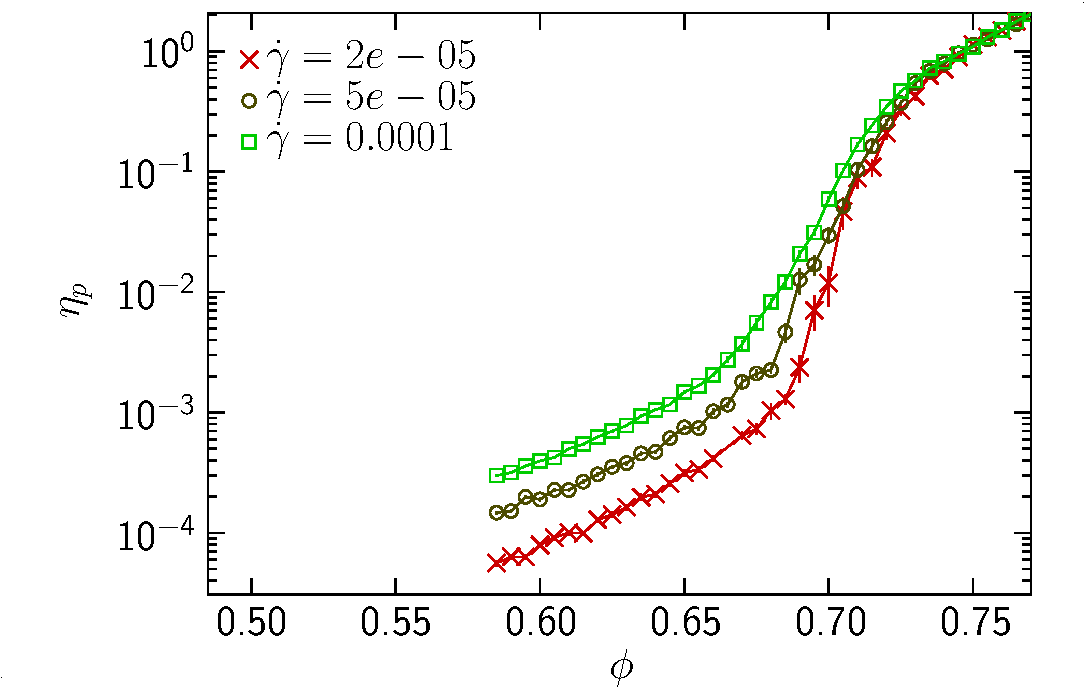
\includegraphics[width=\textwidth]{figures/figs/etap_0064_KDk500_Ml100_EL080}
        \caption{$\alpha=0.8$, $\phi_C\sim0.72$}
        \label{etap_0064_KDk500_Ml100_EL080}
    \end{subfigure}
    \hfill
    \begin{subfigure}[t]{0.32\textwidth}
        \centering
        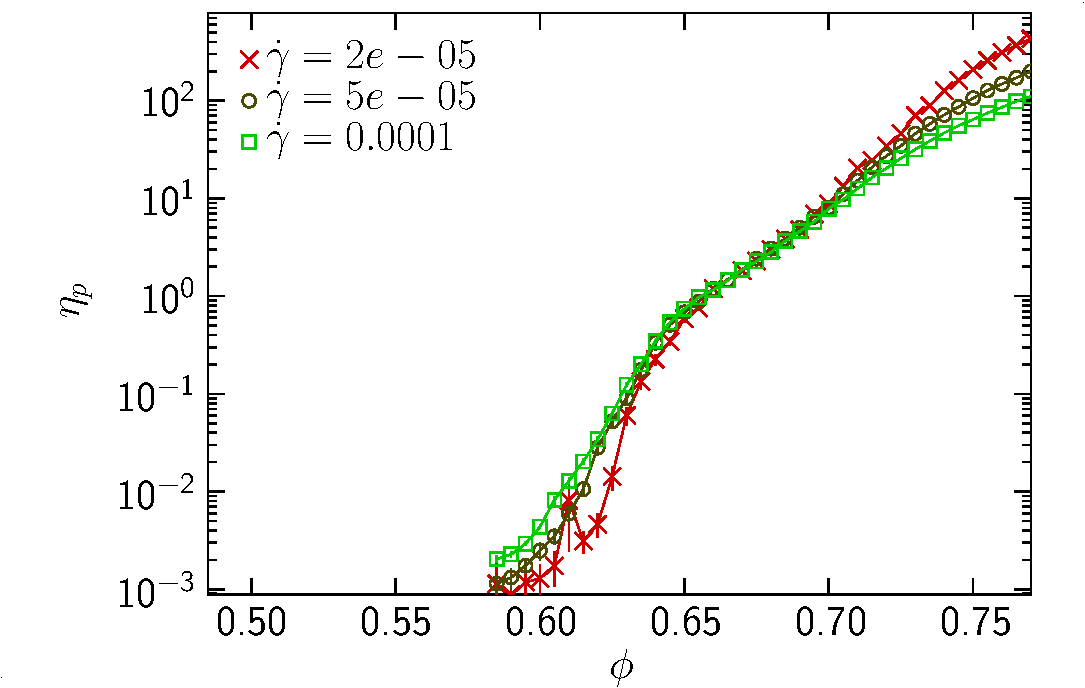
\includegraphics[width=\textwidth]{figures/figs/etap_0064_KDk500_Ml100_EL090}
        \caption{$\alpha=0.9$, $\phi_C\sim0.63$}
        \label{etap_0064_KDk500_Ml100_EL090}
    \end{subfigure}
    \hfill
    \begin{subfigure}[t]{0.32\textwidth}
        \centering
        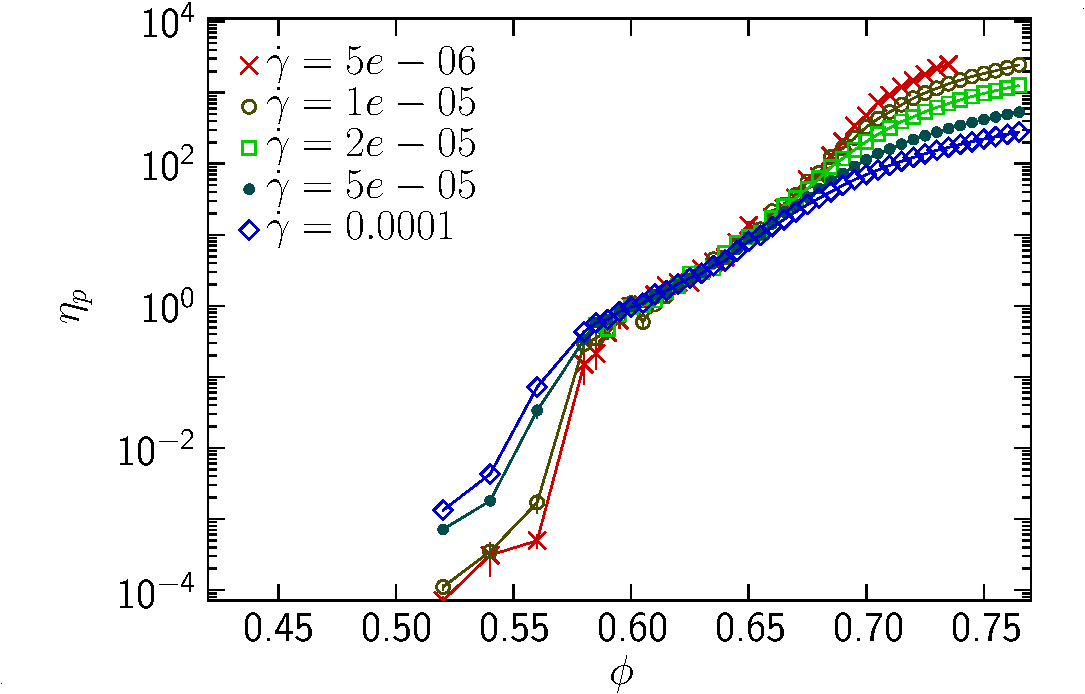
\includegraphics[width=\textwidth]{figures/figs/etap_0064_KDk500_Ml100_EL130}
        \caption{$\alpha=1.3$, $\phi_C\sim0.57$}
        \label{etap_0064_KDk500_Ml100_EL130}
    \end{subfigure}
\caption{Bagnoldian (figures \ref{bp_0064_KDk500_Ml100_EL080}, \ref{bp_0064_KDk500_Ml100_EL090} and \ref{bp_0064_KDk500_Ml100_EL130}) and Newtonian (figures \ref{etap_0064_KDk500_Ml100_EL080}, \ref{etap_0064_KDk500_Ml100_EL090} and \ref{etap_0064_KDk500_Ml100_EL130}) transport coefficients associated to pressure. $N=64,~ k_d=0.5,~ m=1$. We denote $\phi_C$ the transition packing fraction.}
\label{rheo_0064}
\end{figure}

We observe in figure \ref{z_phi_0064_KDk500_Ml100_GDg500} a sharp increase in the average contact number per particle upon increasing the packing fraction. According to the development of part \ref{rheology}, this increase is the sign of a transition from Bagnoldian rheology to Newtonian rheology. We confirm this by determining the Bagnoldian and Newtonian transport coefficients associated to pressure as functions of the packing fraction, and verifying the transitions from a regime to the other occurs at the same packing fractions as the increase of contact number (figure \ref{rheo_0064}).\\

We also observe that the Newtonian transport coefficients become $\dot{\gamma}$-dependent for high enough packing fractions, we will see in part \ref{deviation_hard-core_limit} that this is due to a deviation from the hard-core limit near the jamming transition.\\

Moreover, we can notice that for $1\le\alpha<1.3$ (sphere and prolate spheroids) the transition from the Bagnoldian to the Newtonian regime occurs approximately at the same packing fraction, while for $\alpha=0.8,0.9$ (oblate spheroids) the transition packing fraction $\phi_C$ varies with the aspect ratio and is higher than the value obtained for the former particles.

\subsection{Critical behaviour}

\subsubsection{Deviation from the hard-core limit close to jamming}
\label{deviation_hard-core_limit}

We expect from the development of part \ref{rheology} that the system would display Newtonian rheology sufficiently close to the jamming transition, \textit{i.e.} the Newtonian transport coefficients would be independent of the shear rates at which they are determined. However, this holds only in the hard-core limit.\\

Close to the jamming transition, the overlapping of the particles is non-negligible, hence the deviation from the hard-core limit. This deviation being even more important for higher shear strain rates (figure \ref{etap-phi_0064_KDk500_Ml100_EL130}).

\begin{figure}[h!]
\centering
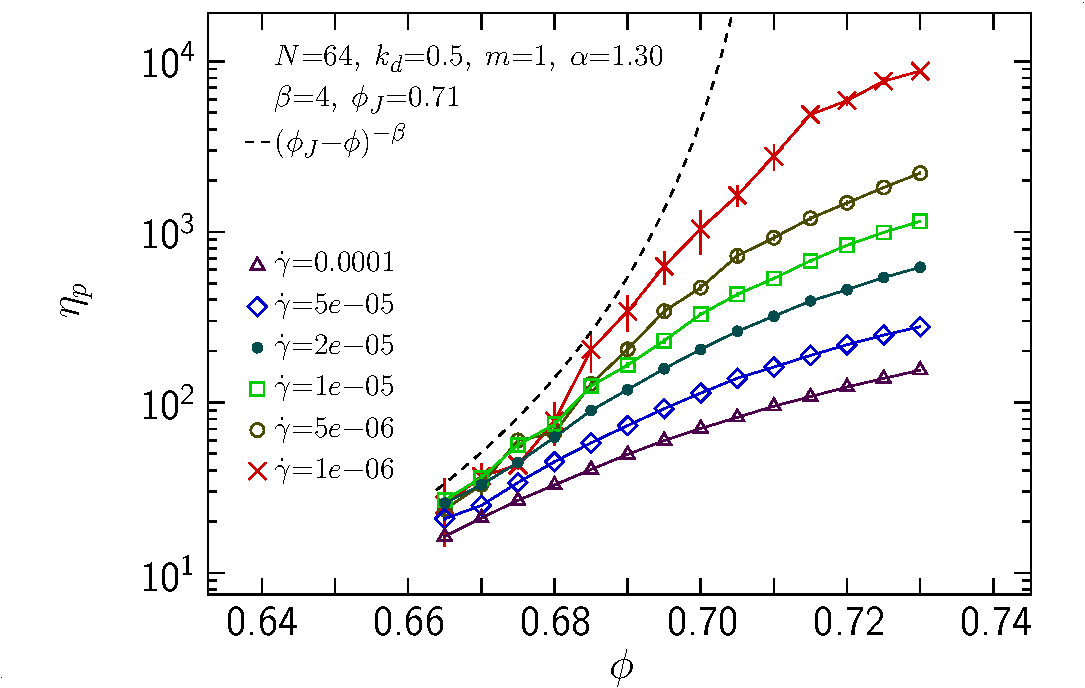
\includegraphics[width=0.6\textwidth]{figures/figs/etap-phi_0064_KDk500_Ml100_EL130}
\caption{Newtonian coefficient of transport associated to pressure as a function of the packing fraction for $\alpha=1.3$.}
\label{etap-phi_0064_KDk500_Ml100_EL130}
\end{figure}

\subsubsection{Effectiveness of scaling}

Figure \ref{p-dphi-scale_0064_KDk500_Ml100_EL130} shows that we have successfully made experimental data from simulations at different density and shear strain rates collapse on a single curve with the method described in part \ref{scaling_analysis}, thus confirming its effectiveness. Scaling exponents from this graph then allowed us to make Newtonian transport coefficients associated to pressure inferred from simulations at different shear rates collapse on a single straight line characterising the critical behaviour described by equation \ref{critical_exponents} for hard-core particles with satisfactory visual precision in figure \ref{etap-phieff_graph_0064_KDk500_Ml100_EL130}.\\

Moreover, we can notice that the mapping parameters determined graphically in figure \ref{etap-phieff_graph_0064_KDk500_Ml100_EL130} ($A=1.9$, $c=0.48$) are close to the values found in \cite{PRL109.108001} for disks ($A=1.53$, $c=0.458$).

\vspace{50pt} % to force the text next subsubsection to display after the figure

\begin{figure}[h!]
\centering
    \begin{subfigure}[t]{0.49\textwidth}
        \centering
        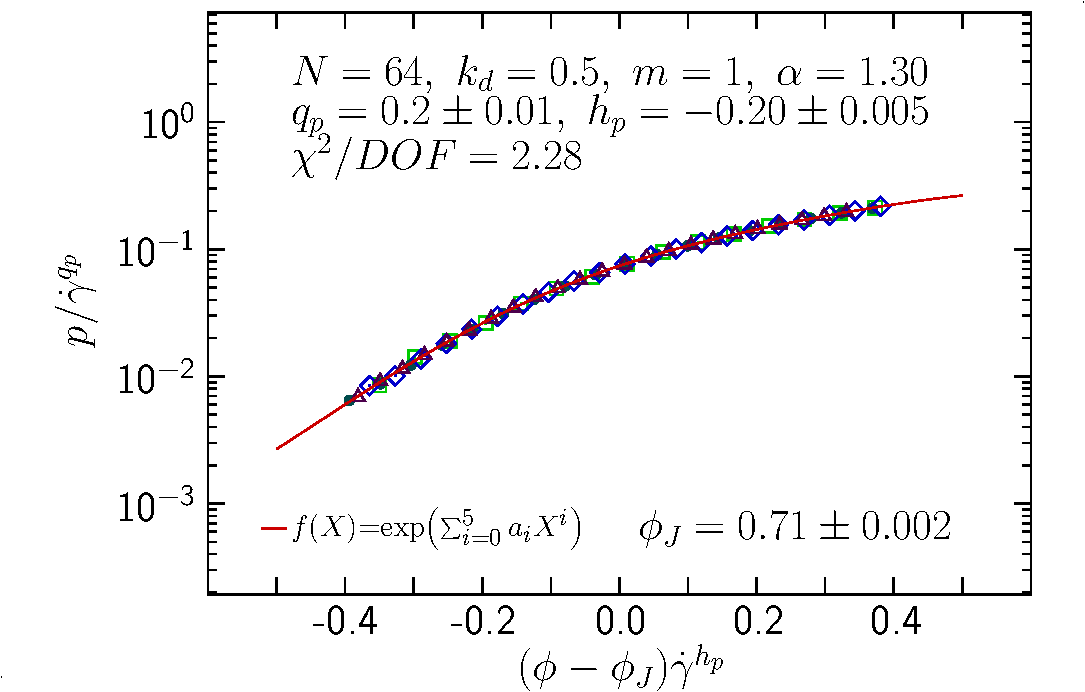
\includegraphics[width=\textwidth]{figures/figs/p-dphi-scale_0064_KDk500_Ml100_EL130}
        \caption{Pressure scaling plot, as described in part \ref{pressure_scaling_method}.}
        \label{p-dphi-scale_0064_KDk500_Ml100_EL130}
    \end{subfigure}
    \hfill
    \begin{subfigure}[t]{0.49\textwidth}
        \centering
        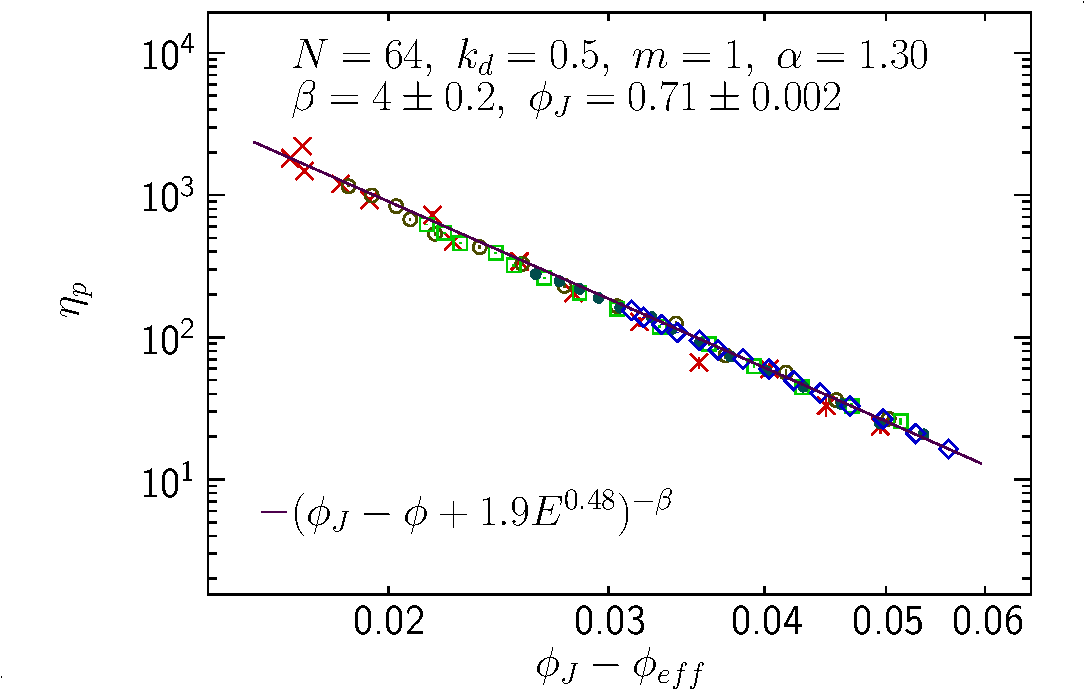
\includegraphics[width=\textwidth]{figures/figs/etap-phieff_graph_0064_KDk500_Ml100_EL130}
        \caption{Newtonian transport coefficient associated to pressure scaling plot, obtained with the soft- to hard-core mapping method described in parts \ref{softtohard} and \ref{softtohardcomplement}. We privileged here the graphical determination of the mapping parameters.}
        \label{etap-phieff_graph_0064_KDk500_Ml100_EL130}
    \end{subfigure}
    \caption{Scaling plots for $\alpha=1.3$.}
    \label{scaling_effectiveness_0064}
\end{figure}

\subsubsection{Jamming density and critical exponent}

From plots such as figure \ref{p-dphi-scale_0064_KDk500_Ml100_EL130} we were able to determine the jamming density and critical exponents for different aspect ratios (see figure \ref{phij_beta_0064}).

\begin{figure}[h!]
\centering
    \begin{subfigure}[t]{0.49\textwidth}
        \centering
        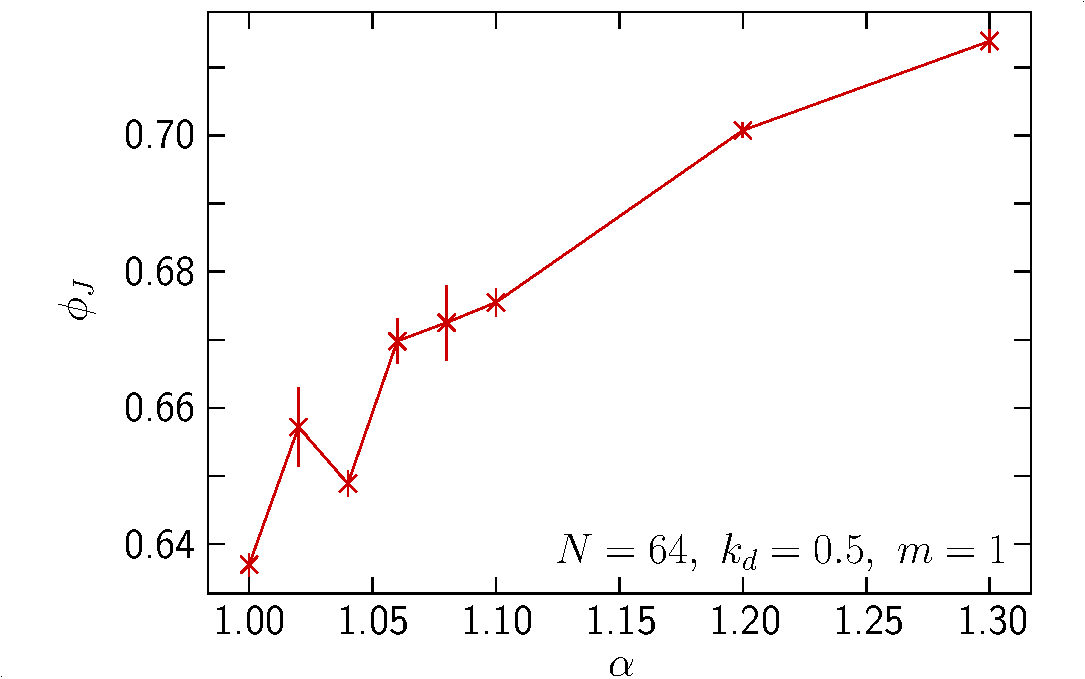
\includegraphics[width=\textwidth]{figures/figs/phij_alpha_0064_KDk500_Ml100}
        \caption{Jamming packing fraction as a function of the aspect ratio.}
        \label{phij_alpha_0064_KDk500_Ml100}
    \end{subfigure}
    \hfill
    \begin{subfigure}[t]{0.49\textwidth}
        \centering
        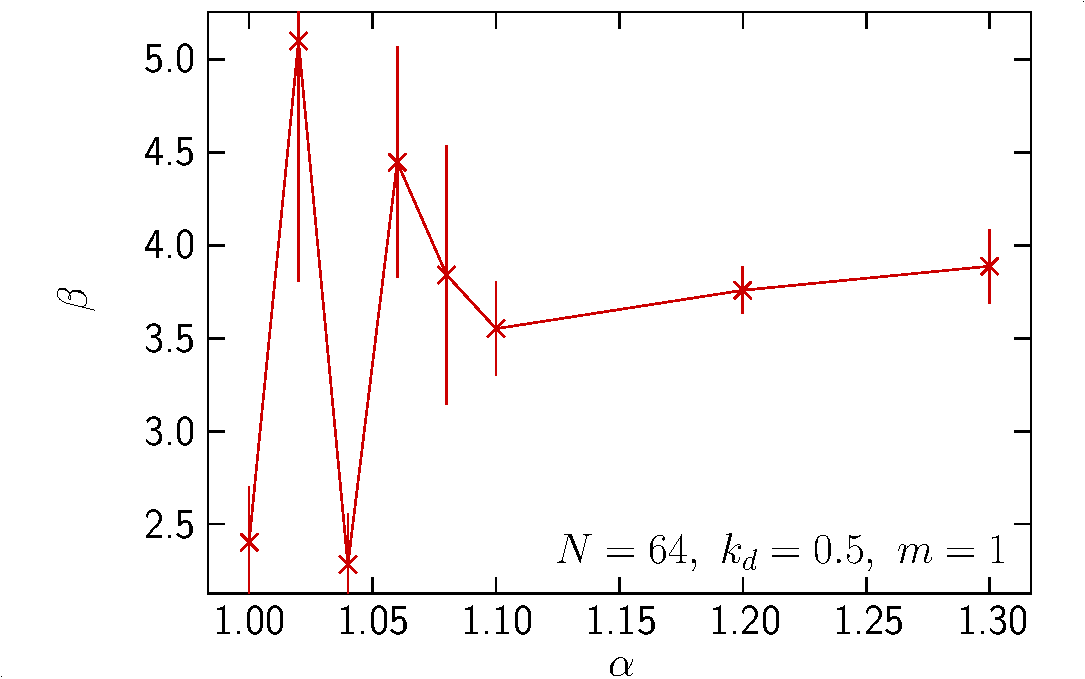
\includegraphics[width=\textwidth]{figures/figs/beta_alpha_0064_KDk500_Ml100}
        \caption{Critical exponent associated to the divergence of the Newtonian transport coefficients as a function of the aspect ratio.}
        \label{beta_alpha_0064_KDk500_Ml100}
    \end{subfigure}
    \caption{Jamming parameters for spheres and prolate spheroids.}
    \label{phij_beta_0064}
\end{figure}

We can first notice that for $\alpha=1$, \textit{i.e.} for spheres, we have $\beta\sim2.5$ which is close to the result of \cite{PRL109.108001} for disks ($\beta=2.58$). Moreover, we have the jamming packing fraction $\phi_J\sim0.64$ close to the random close packing fraction for spheres \cite{donev2004improving}.\\

For the set of aspect ratios considered ($1\le\alpha\le1.3$), we have that the jamming packing fraction is an increasing function of the aspect ratio (figure \ref{phij_alpha_0064_KDk500_Ml100}) -- if we exclude $\alpha=1.04$. This is in accordance with \cite{donev2004improving} which found that $\phi_J$ was an increasing function of the aspect ratio for $1\le\alpha\lesssim1.6$. Simulations with $64$ particles were performed for oblate particles but not close enough to the jamming transition to give $\phi_J$ and $\beta$ with good precision. Nonetheless, we also observed for these particles that the jamming packing fraction would be greater than its value for packings of spheres. More specifically, we estimated $0.7 < \phi_J(\alpha=0.9) < \phi_J(\alpha=0.8)$.\\

It is more difficult to predict the behaviour of the critical exponent $\beta$ from figure \ref{beta_alpha_0064_KDk500_Ml100}. However -- if we exclude $\alpha=1.04$ once again -- we can assume that the critical exponent associated to the divergence of the Newtonian transport coefficients is higher, and has a value close to $\sim 4$, for prolate spheroids than for spheres.

\subsection{Orientation}

Following the claim that shearing breaks the isotropy of space in part \ref{orientational_ordering}, we wished to check if
\begin{itemize}
\item[(i)] spheroids tend to angle themselves in a particular direction,
\item[(ii)] the orientation of the spheroids is correlated.
\end{itemize}

\subsubsection{Direction of orientation}

We denote $O_i$ the mean over configurations of the system of the square of the projection of the axis of symmetry of the spheroid on the $i^{\text{th}}$ axis, with then $\sum_{i=1}^3 O_i^2 = 1$ and the $0^{\text{th}}$ and $1^{\text{st}}$ axis corresponding the directions of the shear and the gradient of shear velocity respectively.

\begin{figure}[h!]
\centering
    \begin{subfigure}[t]{0.49\textwidth}
        \centering
        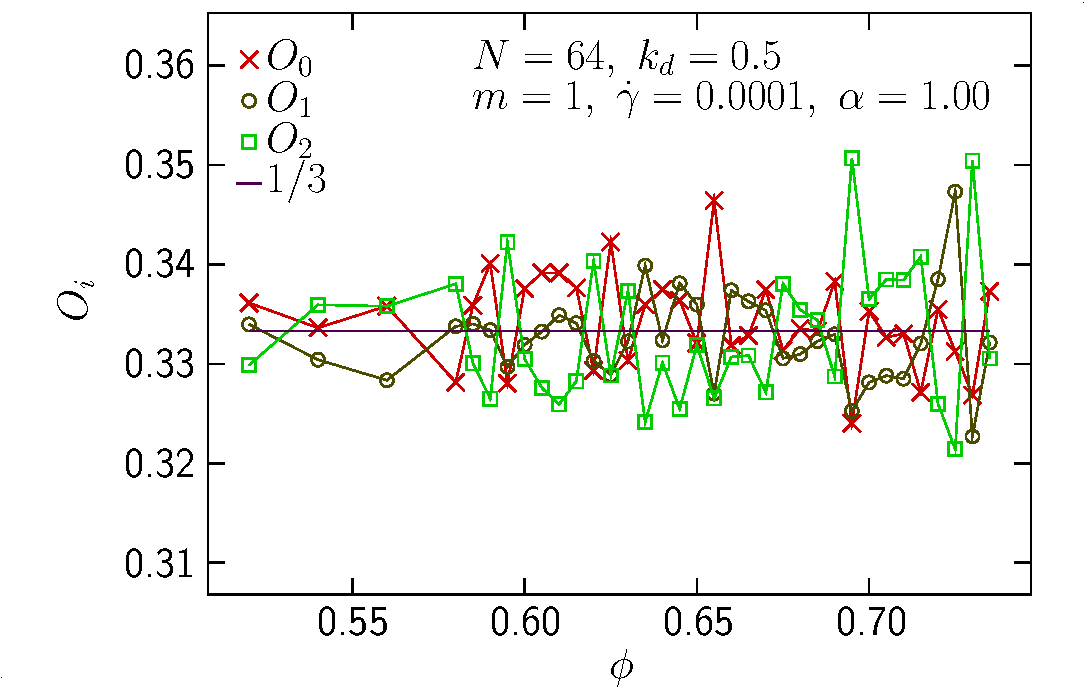
\includegraphics[width=\textwidth]{figures/figs/ori_phi_0064_KDk500_Ml100_GDh100_EL100}
        \caption{$\alpha=1$. Straight line corresponds to $O_i=1/3$.}
        \label{ori_phi_0064_KDk500_Ml100_GDh100_EL100}
    \end{subfigure}
    \hfill
    \begin{subfigure}[t]{0.49\textwidth}
        \centering
        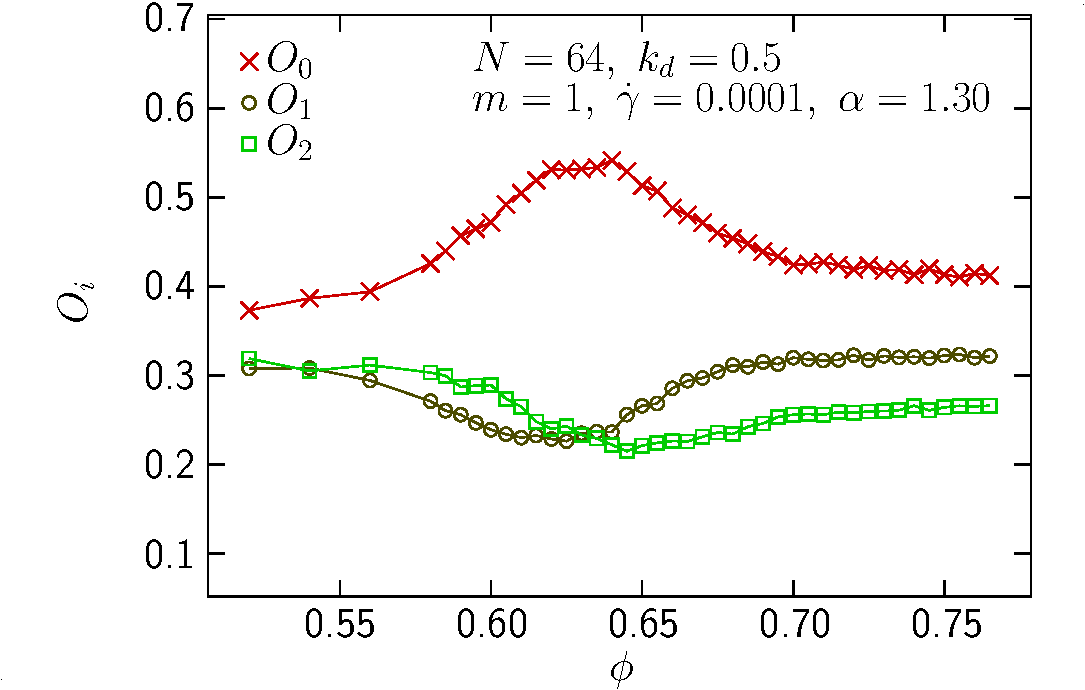
\includegraphics[width=\textwidth]{figures/figs/ori_phi_0064_KDk500_Ml100_GDh100_EL130}
        \caption{$\alpha=1.3$}
        \label{ori_phi_0064_KDk500_Ml100_GDh100_EL130}
    \end{subfigure}
    \caption{Mean squared orientation of the axis of symmetry of the particles.}
    \label{ori_phi_0064}
\end{figure}

We expect that all orientations are equivalent for spheres, which is confirmed by figure \ref{ori_phi_0064_KDk500_Ml100_GDh100_EL100} in which the projections do not show any particular behaviours.\\

For spheroids we see that the $0^{\text{th}}$ direction may be privileged since the mean squared projection of the axis of symmetry on this direction describes a well-defined peak around a given packing fraction while the projections on the other directions reach their minimum around this same packing fraction but both at different densities though (figure \ref{ori_phi_0064_KDk500_Ml100_GDh100_EL130}).\\

Moreover, since the projection curves on the $1^{\text{st}}$ and $2^{\text{nd}}$ directions are well-defined -- contrarily to the curves in figure \ref{ori_phi_0064_KDk500_Ml100_GDh100_EL100} -- we cannot say that the shear direction is the only relevant direction in our system.

\myparagraph{Prolate spheroids}

\begin{figure}[h!]
\centering
    \begin{subfigure}[t]{0.49\textwidth}
        \centering
        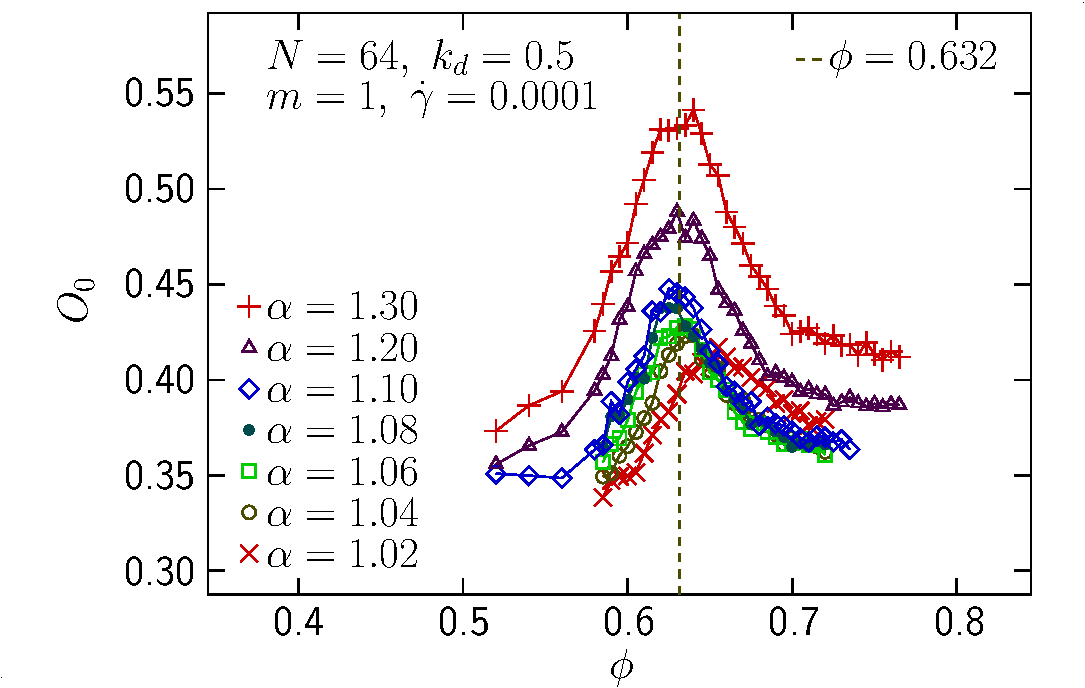
\includegraphics[width=\textwidth]{figures/figs/ori0_phi_prolate_0064_KDk500_Ml100_GDh100}
        \caption{Raw projections.}
        \label{ori0_phi_prolate_0064_KDk500_Ml100_GDh100}
    \end{subfigure}
    \hfill
    \begin{subfigure}[t]{0.49\textwidth}
        \centering
        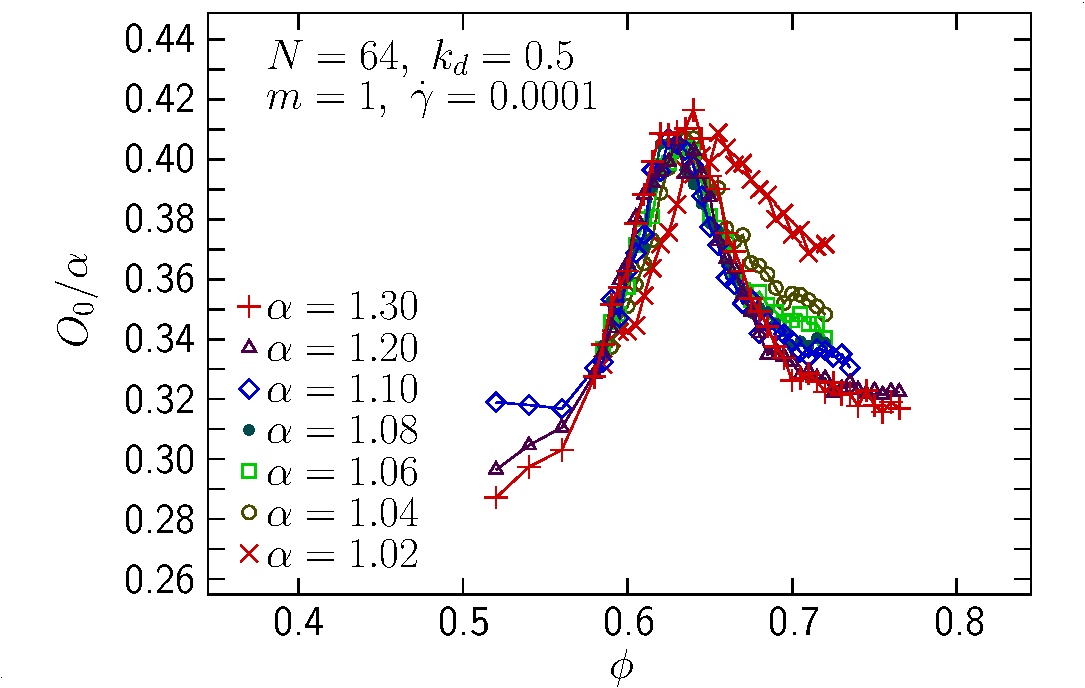
\includegraphics[width=\textwidth]{figures/figs/ori0al_phi_prolate_0064_KDk500_Ml100_GDh100}
        \caption{Projections ratioed with the aspect ratio.}
        \label{ori0al_phi_prolate_0064_KDk500_Ml100_GDh100}
    \end{subfigure}
    \caption{Mean of the squared projection of the axis of symmetry of the particles on shear direction as a function of the packing fraction.}
    \label{ori_phi_0064}
\end{figure}

For all the aspect ratios greater than one we have tested, the mean projection of the axis of symmetry of the particles on the shear direction reaches a well-defined peak (figure \ref{ori0_phi_prolate_0064_KDk500_Ml100_GDh100}). We have that the height of this peak is approximately proportional to the aspect ratio $\alpha$ (figure \ref{ori0al_phi_prolate_0064_KDk500_Ml100_GDh100}).\\

We can notice that the packing fractions at which these peaks appear are somewhat lower than the jamming densities corresponding to the aspect ratios. Indeed, we can read $\phi_J(\alpha>1) \gtrsim 0.65$ from figure \ref{phij_alpha_0064_KDk500_Ml100}. They are also undoubtedly higher than the rheological transition packing fractions (figure \ref{z_phi_0064_KDk500_Ml100_GDg500}) and therefore these peaks do not correspond to any transition or phenomenon we have already described or expected.\\

Furthermore, what figure \ref{ori0al_phi_prolate_0064_KDk500_Ml100_GDh100} also shows is that the position of the peak is much less dependent of the aspect ratio than the jamming density, and even seems not to vary at all -- if we exclude $\alpha=1.02$. However, it should be delicate to extrapolate such a result to hard-core particles since the overlaps are not negligible this close to the jamming transition, which suggests that we should rather be attentive to these variables as functions of the effective packing fraction (figure \ref{ori_phieff_0064}).

\begin{figure}[h!]
\centering
    \begin{subfigure}[t]{0.49\textwidth}
        \centering
        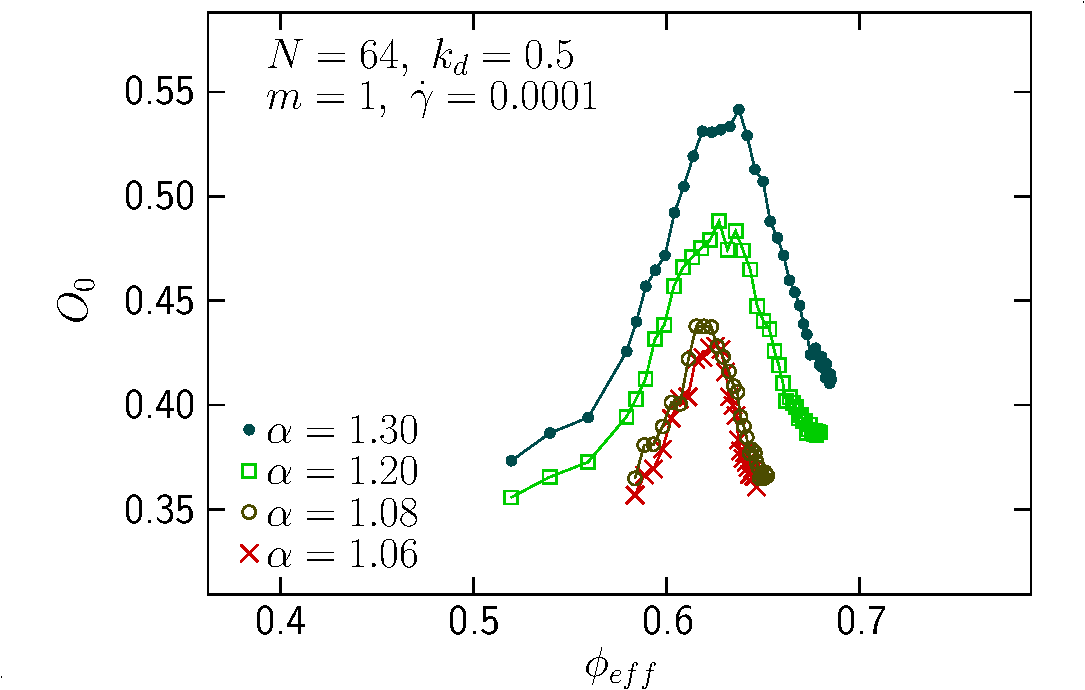
\includegraphics[width=\textwidth]{figures/figs/ori0_phieff_0064_KDk500_Ml100_GDh100}
        \caption{Raw projections.}
        \label{ori0_phieff_prolate_0064_KDk500_Ml100_GDh100}
    \end{subfigure}
    \hfill
    \begin{subfigure}[t]{0.49\textwidth}
        \centering
        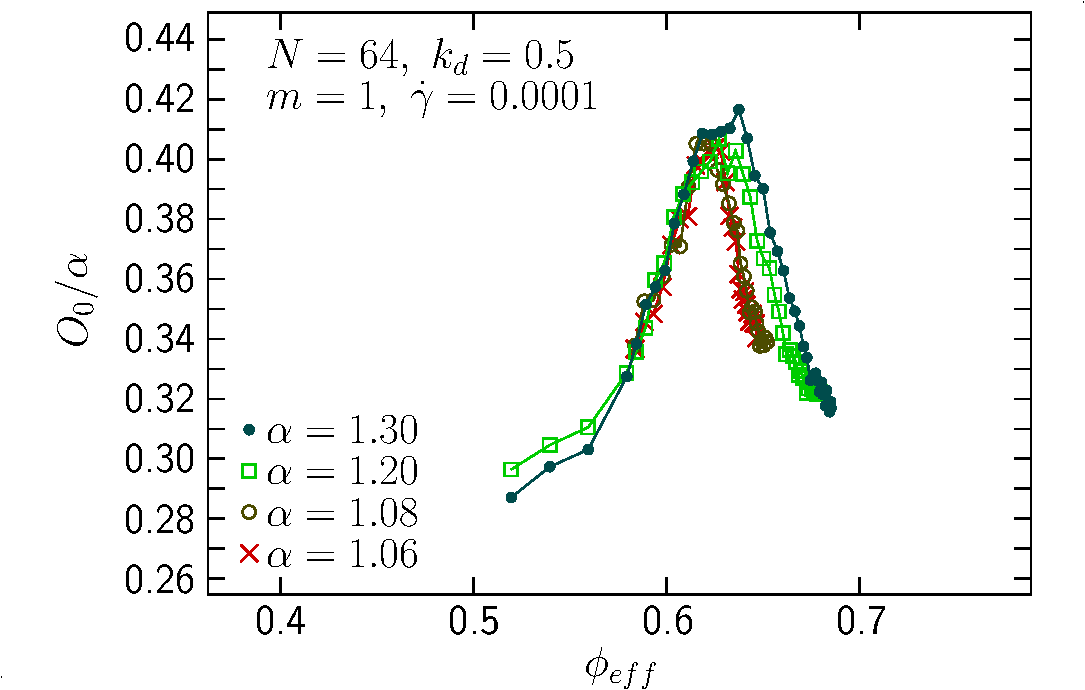
\includegraphics[width=\textwidth]{figures/figs/ori0al_phieff_0064_KDk500_Ml100_GDh100}
        \caption{Projections ratioed with the aspect ratio.}
        \label{ori0al_phieff_prolate_0064_KDk500_Ml100_GDh100}
    \end{subfigure}
    \caption{Mean projection of the axis of symmetry of the particles on the direction of the shear rate as a function of the effective packing fraction. We only show the aspect ratios for which the soft- to hard-core mapping gives a satisfactory visual precision.}
    \label{ori_phieff_0064}
\end{figure}

A quick visual analysis of figure \ref{ori_phieff_0064} shows that the effective packing fraction at which the projection of the axis of symmetry of prolate spheroids on the shear direction reaches its peak is also much less dependent of the aspect ratio than the jamming packing fraction is.\\

We can also be interested in knowing if the observations on the projection of the axis of symmetry on the shear direction (figure \ref{ori_phi_0064}) hold for the two other projections (figure \ref{ori12_phi_0064}).

\begin{figure}[h!]
\centering
    \begin{subfigure}[t]{0.49\textwidth}
        \centering
        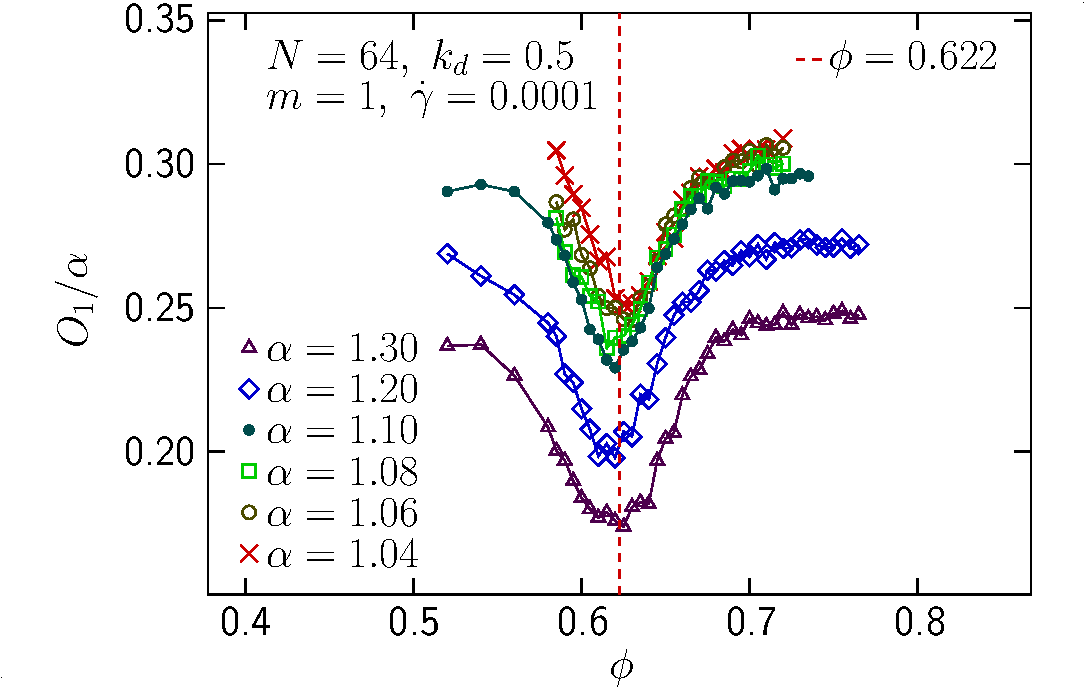
\includegraphics[width=\textwidth]{figures/figs/ori1al_phi_0064_KDk500_Ml100_GDh100}
        \caption{Projection on the direction of the gradient of shear rate.}
        \label{ori1al_phi_0064_KDk500_Ml100_GDh100}
    \end{subfigure}
    \hfill
    \begin{subfigure}[t]{0.49\textwidth}
        \centering
        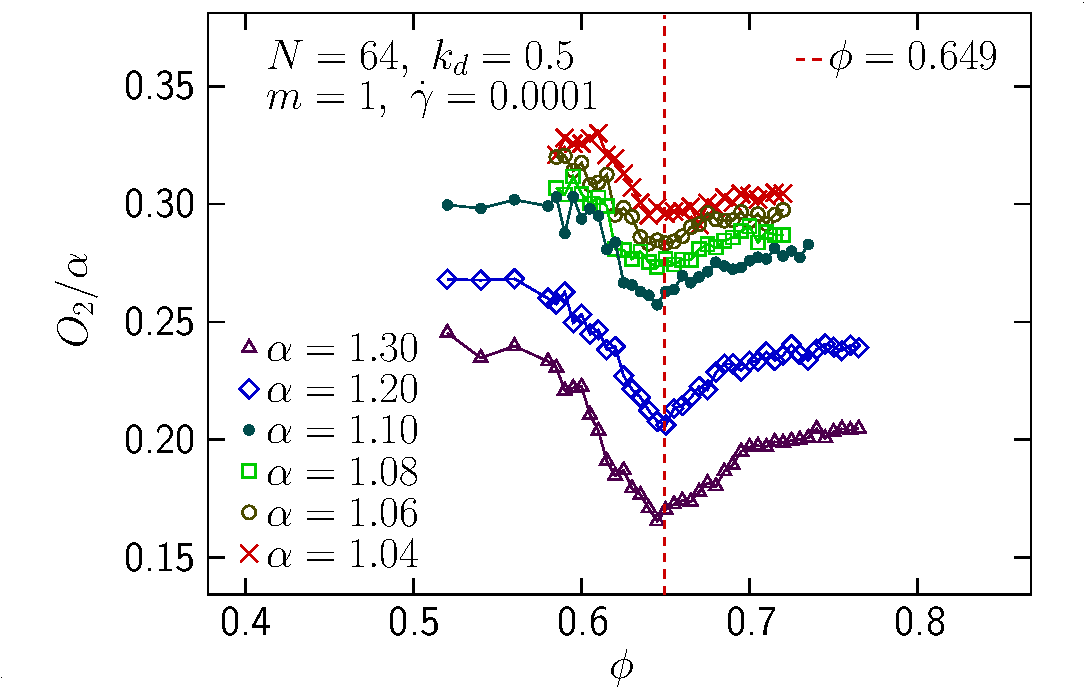
\includegraphics[width=\textwidth]{figures/figs/ori2al_phi_0064_KDk500_Ml100_GDh100}
        \caption{Projection on the $2^{\text{nd}}$ direction.}
        \label{ori2al_phi_0064_KDk500_Ml100_GDh100}
    \end{subfigure}
    \caption{Mean of the squared projections of the axis of symmetry of the particles as functions of the packing fraction.}
    \label{ori12_phi_0064}
\end{figure}

As expected from figure \ref{ori_phi_0064_KDk500_Ml100_GDh100_EL130}, both projections reach a minimum which position, for a given aspect ratio, depends on the axis of projection. Visually, we can claim that the packing fraction at which $O_0$ reaches its maximum (see figure \ref{ori_phi_0064}) is higher than the packing fraction at which $O_1$ reaches its minimum and lower than than the packing fraction at which $O_2$ reaches its minimum, in accordance with figure \ref{ori_phi_0064_KDk500_Ml100_GDh100_EL130}.\\

There is no relation of proportionality between the depths of the minimums and the aspect ratio for these projections, contrarily to what we would have expected from figure \ref{ori0al_phi_prolate_0064_KDk500_Ml100_GDh100}. Moreover, we observe that for $1<\alpha<1.3$, \textit{i.e.} for not too elongated prolate spheroids, the minimum reached by $O_1$ is lower than the minimum reached by $O_2$.\\

We still observe that the positions of the minimums are much less dependent of the aspect ratio than the jamming density, as we observed for the projection on the shear direction.

\myparagraph{Oblate spheroids}

\begin{figure}[h!]
\centering
    \begin{subfigure}[t]{0.49\textwidth}
        \centering
        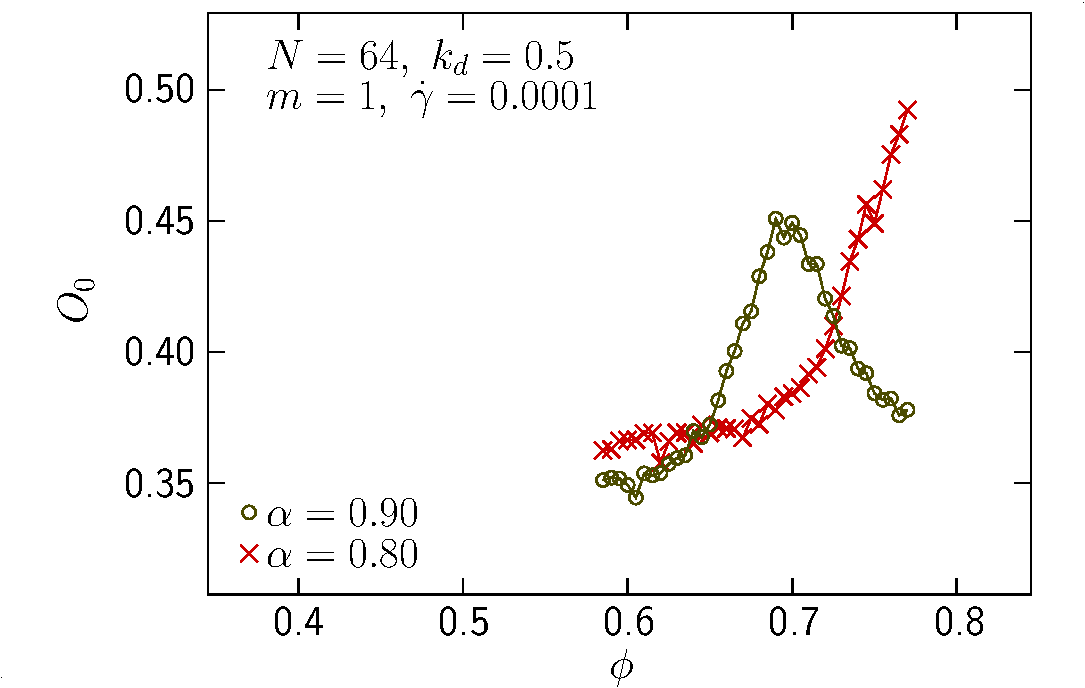
\includegraphics[width=\textwidth]{figures/figs/ori0_phi_oblate_0064_KDk500_Ml100_GDh100}
        \caption{Raw projections.}
        \label{ori0_phi_oblate_0064_KDk500_Ml100_GDh100}
    \end{subfigure}
    \hfill
    \begin{subfigure}[t]{0.49\textwidth}
        \centering
        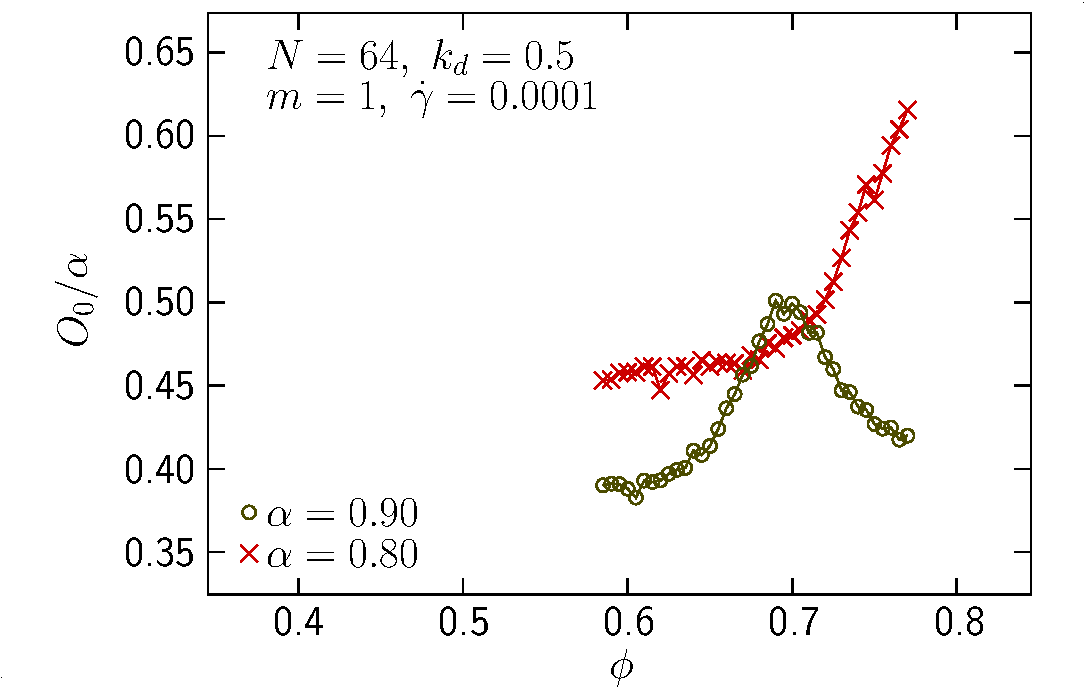
\includegraphics[width=\textwidth]{figures/figs/ori0al_phi_oblate_0064_KDk500_Ml100_GDh100}
        \caption{Projections ratioed with the aspect ratio.}
        \label{ori0al_phi_oblate_0064_KDk500_Ml100_GDh100}
    \end{subfigure}
    \caption{Mean projection of the axis of symmetry of the particles on the direction of the shear rate as a function of the packing fraction.}
    \label{ori_phi_oblate_0064}
\end{figure}

We do not have data at sufficiently high packing fraction to observe the peak of the projection of the axis of symmetry on the shear direction for $\alpha=0.8$, however the data presented in figure \ref{ori_phi_oblate_0064} clearly shows that we should expect for oblate spheroids that the position of the peak strongly depends on the aspect ratio and moreover that its height is not proportional to the aspect ratio, contrarily to prolate spheroids.\\

This, in addition to the fact that the rheological transition also does not appear at the same packing fractions for oblate spheroids contrarily to prolate spheroids (part \ref{preliminary_rheological_transition}), shows that the behaviour of packings of prolate and oblate spheroids is very different, and suggest we may expect the mechanisms governing the jamming transition for these types of particles to be different.

\begin{figure}[h!]
\centering
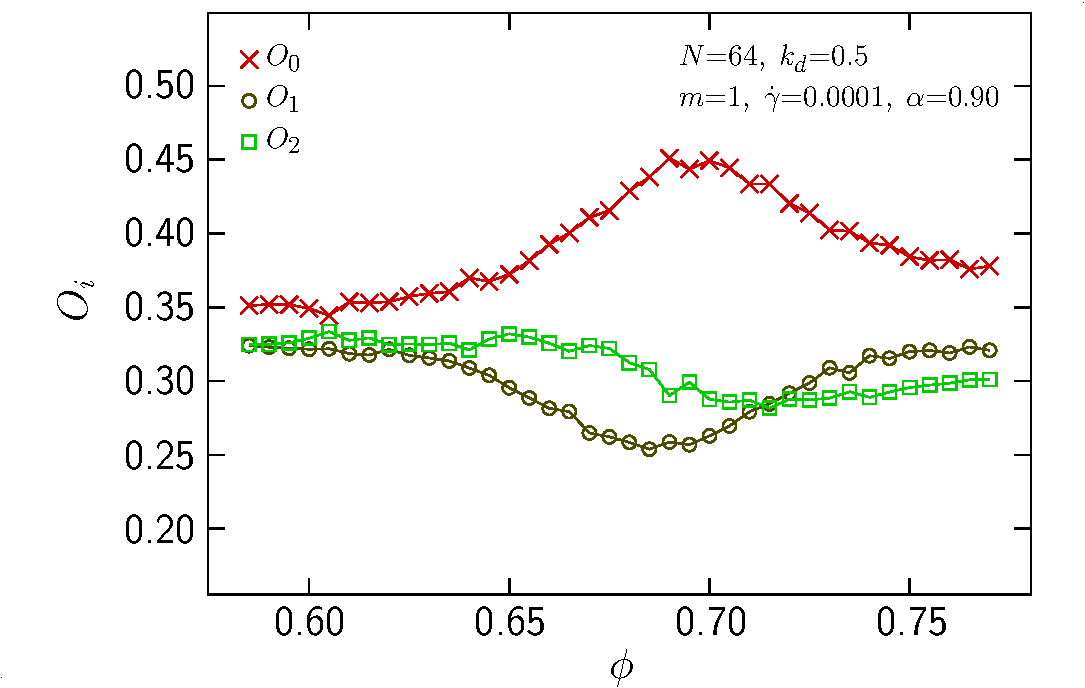
\includegraphics[width=0.6\textwidth]{figures/figs/ori_phi_0064_KDk500_Ml100_GDh100_EL090}
\caption{Mean squared orientation of the axis of symmetry of the particles for $\alpha=0.8$.}
\label{ori_phi_0064_KDk500_Ml100_GDh100_EL090}
\end{figure}

Otherwise, we expect the observations we have made about the projections on all axis as functions of the packing fraction for a given aspect ration (see figure \ref{ori_phi_0064_KDk500_Ml100_GDh100_EL130}) to remain valid for oblate spheroids (see figure \ref{ori_phi_0064_KDk500_Ml100_GDh100_EL090}).

\subsubsection{Correlation}

$\mathcal{C}_{ij}$ is a function which increases with increasing correlation between the orientations of the spheroids.

\myparagraph{Prolate spheroids}

\begin{figure}[h!]
\centering
    \begin{subfigure}[t]{0.49\textwidth}
        \centering
        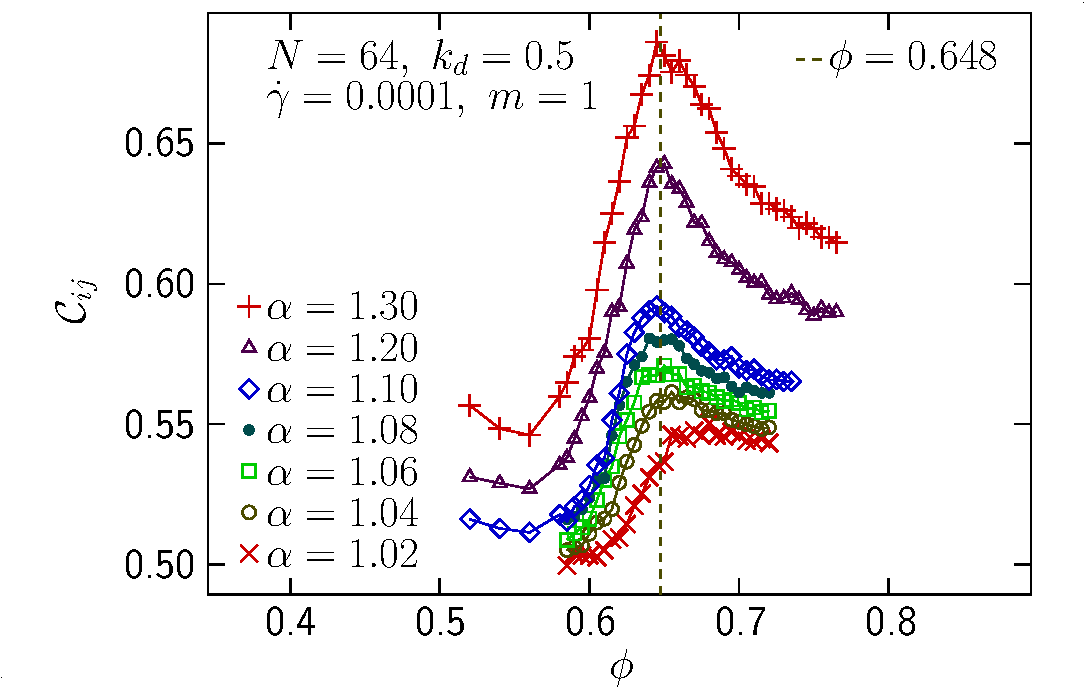
\includegraphics[width=\textwidth]{figures/figs/orij_phi_prolate_0064_KDk500_Ml100_GDh100}
        \caption{Raw correlation function.}
        \label{orij_phi_prolate_0064_KDk500_Ml100_GDh100}
    \end{subfigure}
    \hfill
    \begin{subfigure}[t]{0.49\textwidth}
        \centering
        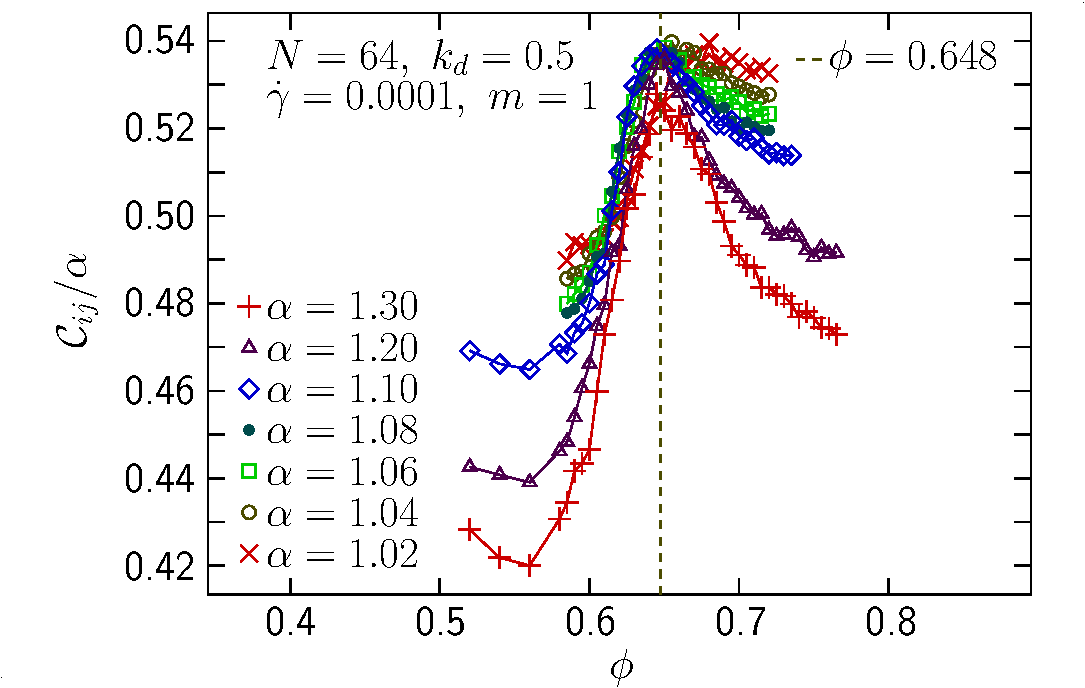
\includegraphics[width=\textwidth]{figures/figs/orijal_phi_prolate_0064_KDk500_Ml100_GDh100}
        \caption{Correlation function ratioed with the aspect ratio.}
        \label{orijal_phi_prolate_0064_KDk500_Ml100_GDh100}
    \end{subfigure}
    \caption{Orientation correlation as a function of the packing fraction.}
    \label{orij_phi_0064}
\end{figure}

As the mean squared projection of the axis of symmetry on the shear direction (see figure \ref{ori_phi_0064}), the correlation function $\mathcal{C}_{ij}$ reaches a peak which height is proportional to the aspect ratio if we let aside $\alpha=1.3$, \textit{i.e.} if we only consider not too elongated prolate spheroids. Moreover, the position of this peak is much less dependent of the aspect ratio than the jamming density (see figure \ref{orij_phi_0064}).\\

However, despite the striking resemblance of the aforementioned figures, we have that $\mathcal{C}_{ij}$ reaches its maximum at a packing fraction slightly higher than the packing fraction at which $O_0$ reaches its. Indeed, it rather seems to correspond to the packing fraction rather at which $O_2$ reaches its minimum (see figure \ref{ori2al_phi_0064_KDk500_Ml100_GDh100}).

\myparagraph{Oblate spheroids}

\begin{figure}[h!]
\centering
    \begin{subfigure}[t]{0.49\textwidth}
        \centering
        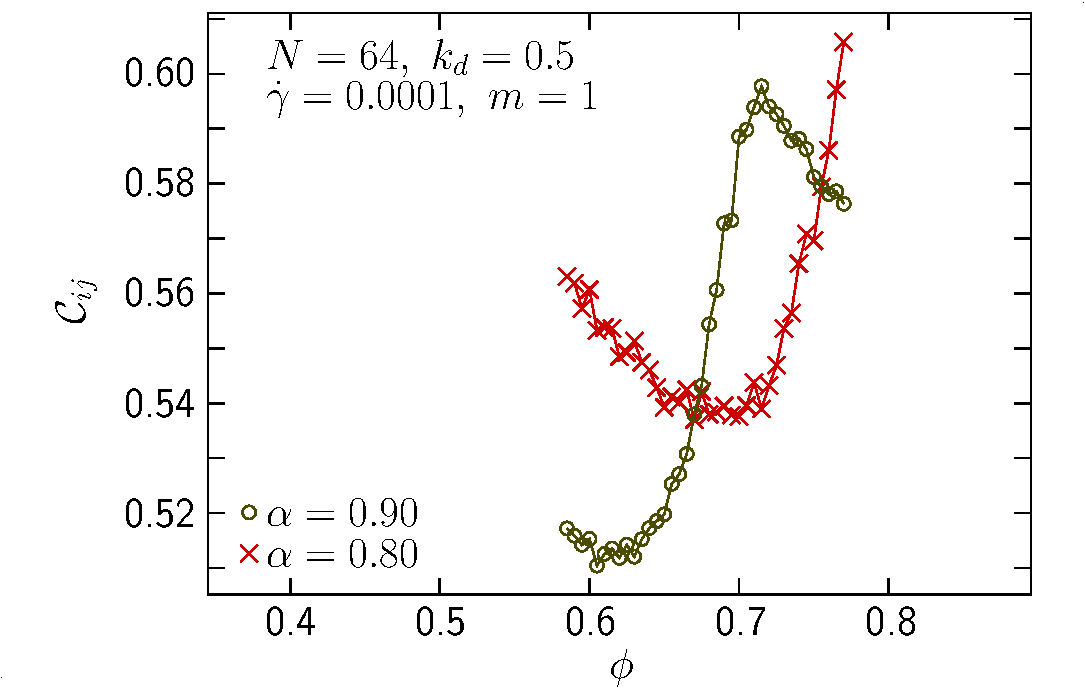
\includegraphics[width=\textwidth]{figures/figs/orij_phi_oblate_0064_KDk500_Ml100_GDh100}
        \caption{Raw correlation function.}
        \label{orij_phi_oblate_0064_KDk500_Ml100_GDh100}
    \end{subfigure}
    \hfill
    \begin{subfigure}[t]{0.49\textwidth}
        \centering
        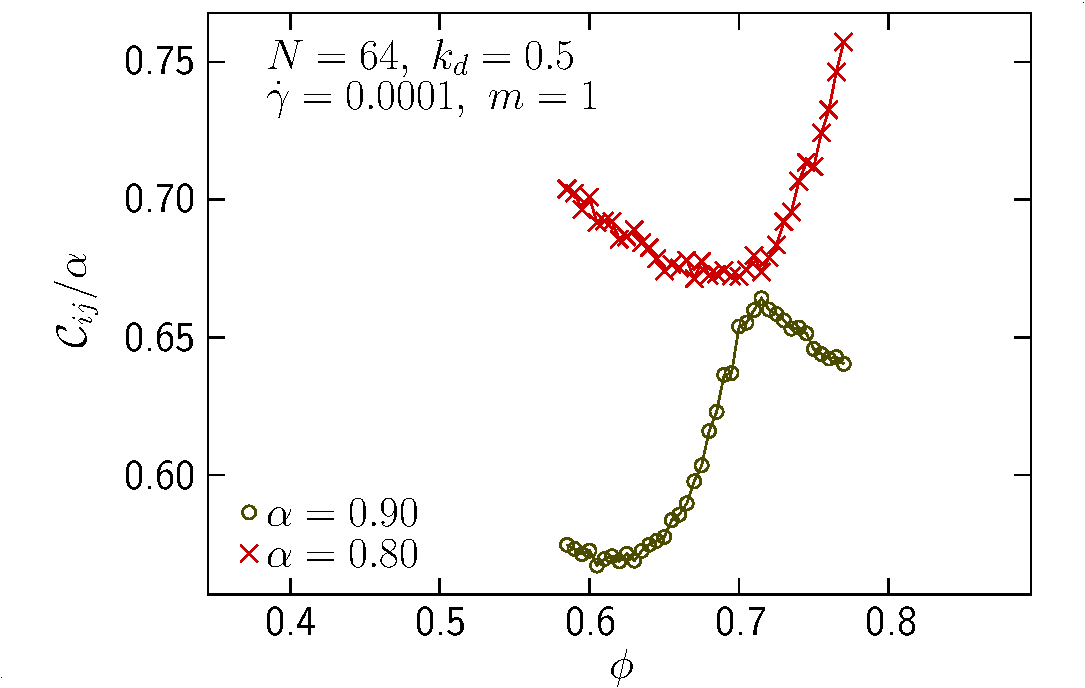
\includegraphics[width=\textwidth]{figures/figs/orijal_phi_oblate_0064_KDk500_Ml100_GDh100}
        \caption{Correlation function ratioed with the aspect ratio.}
        \label{orijal_phi_oblate_0064_KDk500_Ml100_GDh100}
    \end{subfigure}
    \caption{Orientation correlation as a function of the packing fraction.}
    \label{orij_phi_ob_0064}
\end{figure}

As for the projection of the axis of symmetry on the shear direction for oblate particles (see figure \ref{ori_phi_oblate_0064}), we observe here that the position of the peak of correlation function strongly depends on the aspect ratio for oblate particles (see figure \ref{orij_phi_ob_0064}), contrarily to prolate particles (see figure \ref{orij_phi_0064}) -- even though data at higher packing fractions and for more aspect ratios would be needed.\\

Moreover, and still in accordance to what we have observed for the aforementioned projection, there is relation of proportionality between the value of the maximum of the correlation function and the aspect ratio for oblate particles.

\section{Dominance of the elastic pressure}

We claimed in part \ref{pressure_sheared_packing} that the elastic part of the pressure, $p_{\text{el}}$, was the main contribution to the total pressure, $p$.

\begin{figure}[h!]
\centering
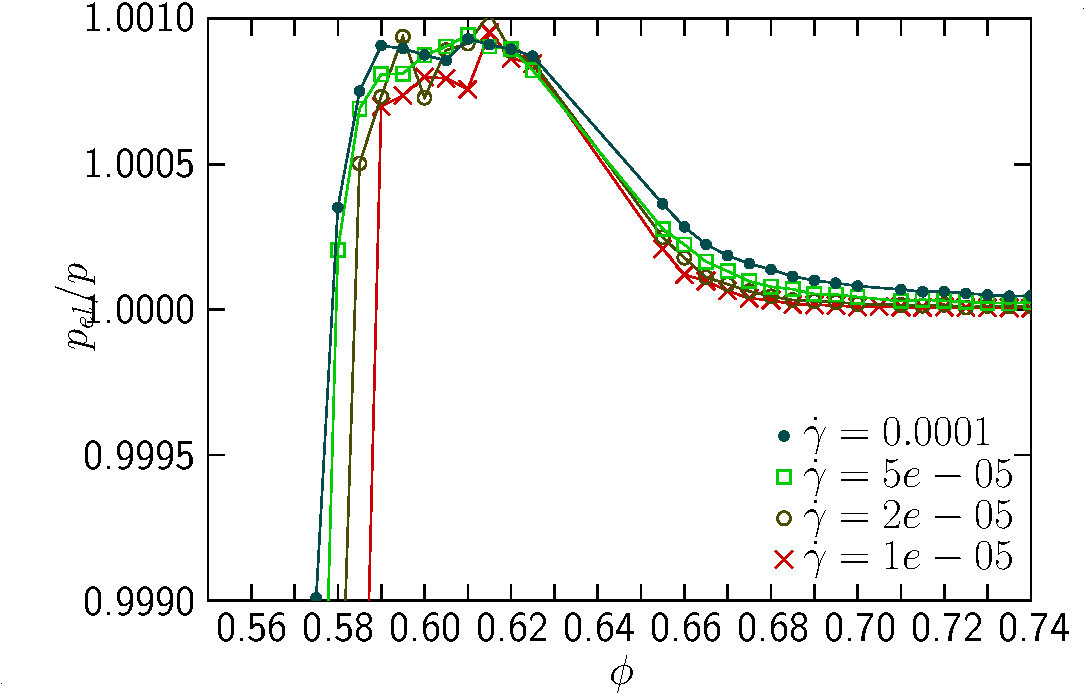
\includegraphics[width=0.6\textwidth]{figures/figs/pe_ptot-zoom-phi}
\caption{Ratio of the elastic pressure $p_{\text{el}}$ and the total pressure $p$.}
\label{pe_ptot-zoom-phi}
\end{figure}

Figure \ref{pe_ptot-zoom-phi} shows that, for $0.59\le\phi\le0.74$, approximating the total pressure by its elastic part gives an error lesser than 0.01\%, thus justifying our claim. We will then use the notation $p$ to designate $p_{\text{el}}$.

\section{Relaxation time}

Relaxation simulations, of which the method is described in part \ref{method_relaxation}, were performed with 16384 particles.\\



\subsection{Exponential decay of the pressure}

\subsection{Scaling of the relaxation time with the packing fraction}

\section{Contact number}

\section{Critical behaviour}

**** MAYBE TELL HOW THE OBSERVATIONS FOR THE RHEOLOGICAL TRANSITION GIVE HINTS ON WHAT'S HAPPENING AT JAMMING (ESPECIALLY WHY JAMMING MIGHT BE GOVERNED BY DIFFERENT MECHANISMS FOR OBLATE AND PROLATE SPHEROIDS) ****

\section{Orientation}

**** PRECISE THAT IT WOULD BE INTERESTING TO CHECK FOR PERIODICITY IN THE ORIENTATION ****

\section{Rotation velocity}

% \addcontentsline{toc}{section}{References}
\bibliographystyle{unsrtnat}
\bibliography{references/biblio}
{\renewcommand{\bibname}{References}\bibliography{references/biblio}}

\end{document}

% \end{cbunit}